\documentclass{aip-cp}


\usepackage[numbers]{natbib}
\usepackage{rotating}
\usepackage{graphicx}
\usepackage{tikz}
\usetikzlibrary{shapes.geometric}
\usetikzlibrary{positioning}
\usetikzlibrary{patterns}
\usetikzlibrary{arrows,decorations.markings}
\usetikzlibrary{spy}

% Document starts
\begin{document}

% Title portion
\title{Simulation and Optimization of Injector Parameters with OpenFOAM and Globalizer Tools}

\author[aff1]{Konstantin Barkalov\corref{cor1}}
\author[aff1]{Ilya Lebedev}
\author[aff2]{Daniil Ryazanov}
\author[aff2]{Sergey Strijak}

\affil[aff1]{Lobachevsky State University of Nizhny Novgorod, Nizhny Novgorod, Russia}
\affil[aff2]{Ivannikov Institute for System Programming of the RAS, Moscow, Russia}
\corresp[cor1]{Corresponding author: konstantin.barkalov@itmm.unn.ru}

\maketitle

\begin{abstract}
The paper presents results of solving the problem of simulation and research of processes taking place in a fuel system injector. Simulation has been carried using tools of the OpenFOAM system. The problem of differential pressure minimization at the injector inlet and outlet was set and solved. This problem was considered as a Lipschitz optimization problem with a black-box type objective function. To solve it, we used an efficient global search algorithm implemented in the Globalizer system.
\end{abstract}

% Head 1
\section{INTRODUCTION}

The problem of designing new engineering objects is inseparably connected with the problem of selecting the best values of item parameters, because the choice of specific values of parameters (with a fixed overall structure) can significantly affect its characteristics.

As engineering objects and conditions of their functioning become more complicated, it results in a significant increase in the complexity of corresponding mathematical models and numerical methods for their analysis. Nowadays, the main (and often the only possible) tool for such analysis is supercomputer simulation of the object's behavior. For this purpose, CAD/CAM/CAE-systems are widely used. A well-known example of open source software of this kind is OpenFOAM, an open platform for numerical simulation of continuum mechanics problems \cite{OpenFOAM}.

In this study, we used the OpenFOAM system to simulate a fuel injector. In the simulation process, the pressure drop at the inlet and outlet of the injector was calculated. The problem of minimizing the pressure drop in order to save fuel by reducing the concentration of combustible substances in the mixture after leaving the ejector was set and solved. The parameters used in the problem included the width of the gap between the injector inlet and the injector outlet.

\section{GLOBAL SEARCH ALGORITHM}


The global optimization problem
\begin{eqnarray}\label{problem}
&\varphi(y^\ast)=\min{\left\{\varphi(y):y\in D\right\}},\\
&D=\left\{y\in R^N: a_j\leq y_j \leq b_j, 1\leq j \leq N \right\},\label{D}
\end{eqnarray}
can serve as a mathematical model for the process of choosing optimum values of parameters $y=(y_1,y_2,...,y_N)$ of the engineering object under consideration.
The choice of the value  $y^*$ that determines the best option  is reduced to an approximate (with some required accuracy) solution of the above optimization problem based on the evaluation of object characteristics for the set of options $y^i\in D, \; 1 \leq i \leq k$, determined by available resources.

The optimal parameter selection problems under consideration are characterized by the fact that the objective function $\varphi(y)$ is not defined analytically; there is only some algorithm to calculate its values at the points of the domain $D$.  In this case, one search trial (calculating the function value in a particular point of the search domain) is a computationally intensive operation \cite{Sergeyev1999,Kvasov2013,Kalyulin2017,Sergeyev2018,Paulavicius2020,Lera2021}.

Multi-extremal optimization problems are essentially more time-consuming in comparison with other types of optimization problems because global optimum is an integral characteristic of the problem to be solved and demands investigation of the whole search domain. As a result, the search for the global optimum is reduced to generating  some covering (grid) in the parameter domain and choosing the best function value on this grid. The amount of calculations can be reduced by creating a non-uniform coverage of the search domain: the grid has to be dense enough in the vicinity of the global optimum and more sparse farther away from the solution being sought.

A typical assumption used in many global optimization methods \cite{Sergeyev2013,Evtushenko2013,Jones2009,Zilinskas2010,Pinter1996,Grishagin2016_1,Sergeyev2021} is the assumption that the objective function $\varphi(y)$ satisfies the Lipschitz condition
\[
\left|\varphi(y_1)-\varphi(y_2)\right|\leq L\left\|y_1-y_2\right\|,\; y_1,y_2 \in D, 0<L<\infty.
\]
% Предположение такого рода является достаточно естественным для многих прикладных задач, поскольку относительные вариации целевой функции, характеризующей моделируемую систему, обычно не могут превышать некоторый порог, определяемый ограниченной энергией изменений в системе.

At the same time, various dimensionality reduction schemes are widely used to reduce the complexity of designing global optimization algorithms. By means of  such schemes, it is possible to reduce solution of multidimensional optimization problems to the solution of one or more nested one-dimensional optimization problems.

One approach to dimensionality reduction is to use Peano-type space filling curves (\textit{evolvents}). Using evolvents $y(x)$, which continuously and uniquely map a unit interval onto a hypercube, reduces the problem of finding the minimum of the function $\varphi(y)$ in the domain $D$ to finding the minimum of a one-dimensional function  on the interval $[0,1]$
\[
\varphi(y^\ast)=\varphi(y(x^\ast))=\min{\left\{\varphi(y(x)): x\in[0,1]\right\}}.
\]
As follows from the properties of the space-filling curve \cite{Sergeyev2013}, the reduced one-dimensional function $\varphi(y(x))$ satisfies a uniform H{\"o}lder condition
\[
\left|\varphi(y(x_1))-\varphi(y(x_2))\right|\leq H\left|x_1-x_2\right|^{1/N}, \; x_1,x_2 \in [0,1],
\]
where the H{\"o}lder constant $H$ is related to the Lipschitz constant $L$ by the relationship $H=2L\sqrt{N+3}$.

The above assumptions and approaches have led to the development of a number of global search algorithms based on the information-statistical approach \cite{Strongin2000}. These algorithms are implemented in the Globalizer software system for solving global optimization problems \cite{globalizerSystem}. Here, we present a scheme of the basic global search algorithm (GSA). This is a Divide-the-Best algorithm \cite{Sergeyev1998}, i.e. it is aimed to conduct a subsequent search trial in the most promising (from the point of view of global minimum detection) search subdomain.

The first two trials are performed at the boundary points of the search domain $x^0 = 0$ and $x^1 = 1$. The selection of the point  $x^{k+1}, \; k \geq 1,$  of any next trial is carried out by the following steps.

Step 1. Renumber the points  $x^1,...,x^k$ of the preceding trials by the lower indices in increasing order of the coordinate values, i.e.
\begin{equation}\label{x_i}
0=x_0<x_1<\dots <x_k<x_{k+1}=1,
\end{equation}
and juxtapose to them the values $z_i=\varphi(y(x_i)), \; 0 \leq i\leq k+1,$  computed at these points.

Step 2. For each interval $(x_{i-1},x_i), \; 1\leq i \leq k+1,$ compute the characteristics $R(i)$ using some formulae.

Step 3. Find the interval $(x_{t-1},x_t),$ with the maximum characteristic \cite{Grishagin1997}
\[
R(t)=\max\{R(i):1 \leq i \leq k+1\}.
\]

Step 4. Execute the next trial in the inner point of the interval  $(x_{t-1},x_t)$, i.e. $x^{k+1} \in (x_{t-1},x_t)$.

Step 5. Check termination condition  $\left(x_t-x_{t-1}\right)^{1/N}<\epsilon$, where $t$ is the number of the interval with the maximum characteristic and $\epsilon>0$ is the predefined accuracy.

The global search algorithm has the folloing interpretation. Using trial points it is possible to design a minorant for which characteristic $R(i)$ is the minimum value of the minorant in the interval $(x_{i-1}, x_i ), 1 \leq i \leq k + 1,$ taken with the opposite sign. Then new trial is carried out in the interval where the global minimizer of the current minorant is situated and the new trial point $x^{k+1}$ coincides with it.

A detailed description of the algorithm, its various modifications (including parallel ones), and the corresponding convergence  theory are presented in \cite{Strongin2000,Barkalov2010,Strongin2020}.
	

\section{NUMERICAL EXPERIMENTS}

The calculations were performed on the computer cluster of the Institute for Systems Programming and the UniHub web-lab \cite{UniHub}. The web-lab architecture is based on the cloud computing model where resources (servers, networks, storage systems, applications, etc.) are provided remotely as a set of different-level services with on-demand servicing.

To carry out numerical experiments, we used the OpenFOAM software package \cite{OpenFOAM}. It is a set of tools for representing, discretizing and manipulating hydrodynamic fields. OpenFOAM also provides methods for solving systems of algebraic equations. The OpenFOAM serves to perform a complete cycle of numerical solution of continuum mechanics problems using the finite volume method: from the mathematical formulation by setting initial conditions, boundary conditions, computational geometry, and computational grid to a representation of the results in the form of hydrodynamic fields.

In our particular case, each iteration of the optimal solution search process was a separate numerical calculation of the hydrodynamic fields. The injector simulation was divided into several key steps:
\begin{enumerate}
\item \textbf{Mathematical formulation}. This includes a procedure for selecting equations describing the dynamics of a fluid or gas, setting boundary conditions and initial conditions. It does not change from iteration to iteration.
\item \textbf{Parameterization}. Selection of varying parameters that will vary from iteration to iteration.
\item \textbf{Generating the geometry and the computational grid}. In line with Parameterization, a procedure for renewing the geometry and computational grid is performed.
\item \textbf{Calculation of hydrodynamic fields}. At each iteration, the system of equations describing fluid dynamics is solved numerically.
\item \textbf{Interpretation}. Physical interpretation of the results after the optimization procedure.
\end{enumerate}

The fluid dynamics for the problem described in this paper is defined by the Navier-Stokes equations for an incompressible fluid:
\[
\nabla \cdot \vec{U} = 0,
\]
\[
\frac{\partial \vec{U}}{\partial t} + \nabla \cdot \left( \vec{U} \otimes \vec{U}\right) - \nabla \cdot \nu \left( \nabla \vec{U} + (\nabla \vec{U})^T\right) = - \frac{1}{\rho} \nabla p,
\]
where $\vec{U}$ is the velocity vector, $\nu$  is the liquid viscosity (assumed constant), $p$  is the overpressure, $\rho$ is the density of the liquid. In this system of equations, there are two unknown variables: $\vec{U}$  and $p$. For each of these variables, initial conditions are set: 
\[
\vec{U}(x,y) = 0,
\]
\[
p(x,y) = 0.
\]
There are three types of boundaries in the computational domain; special boundary conditions are set on each of them. 
On a rigid wall:
\[
\nabla p \cdot \vec{n} = 0,
\]
\[
\vec{U} = 0.
\]
At the entrance to the computational domain:
\[
\nabla p \cdot \vec{n} = 0,
\]
\[
\vec{U} = \vec{U_i}.
\]
At the exit of the computational domain:
\[
 p = 0,
\]
\[
\vec{U} = \vec{U_o}.
\]

The geometric representation of the computational domain is shown in Figure 1, with the parameterization points highlighted in red. The geometry is parametrized by increasing the distance between the red points symmetrically with respect to the channel centreline. 
%Таким образом, в задаче имеется один варьируемый параметр (диаметр сечения канала в его средней части), значения которого изменяются в диапазоне $[0,10]$.

\begin{figure}%[ht]
%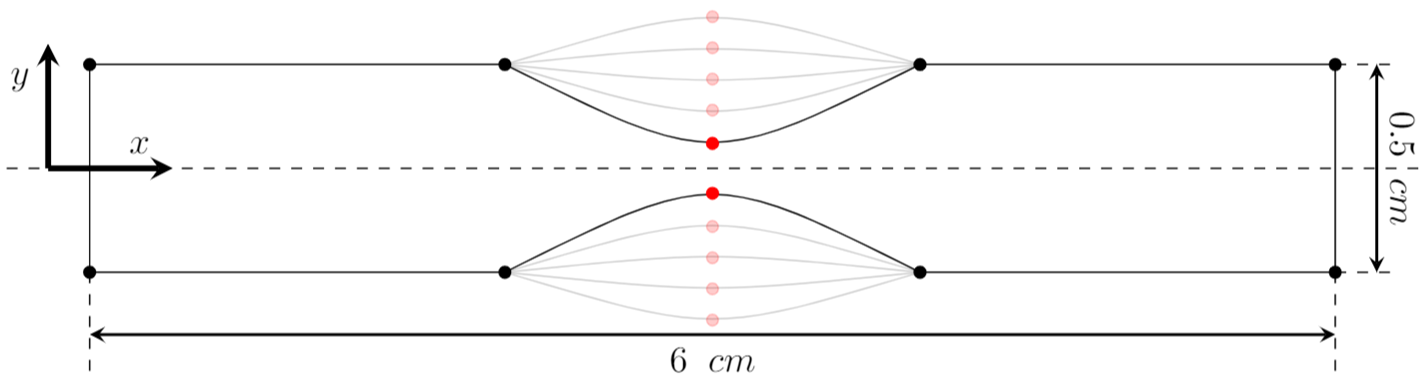
\includegraphics[width=1.0\linewidth]{fig1.png}

    \centering
    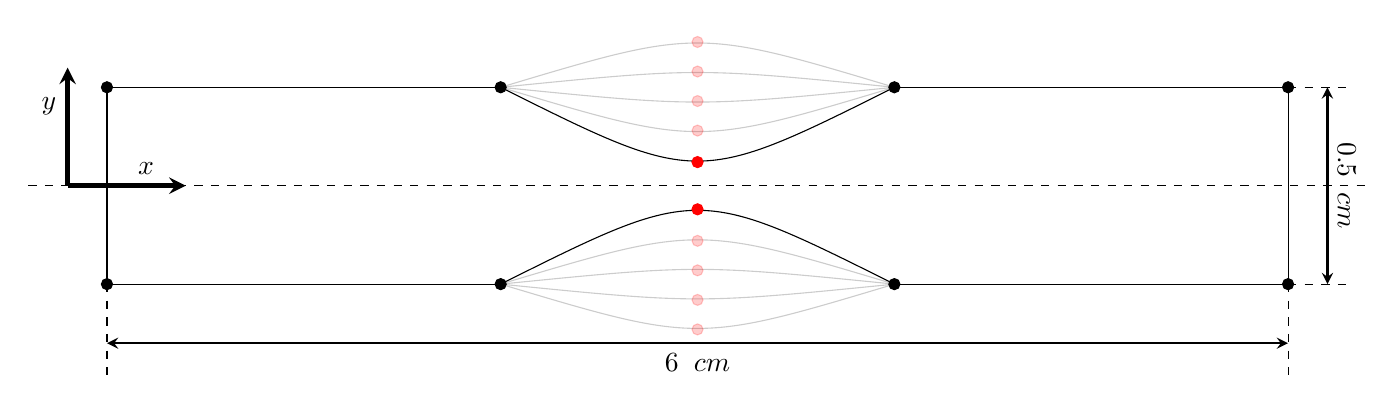
\begin{tikzpicture}[scale=0.5,>=stealth]
         \draw (-5,-2.5,0)--(-15,-2.5,0)--(-15,2.5,0)--(-5,2.5,0.0);%--(0,0.5,0.0)--(5,2.5,0)--(15,2.5,0)--(15,-2.5,0);
         \draw (-5,-2.5) .. controls (0,0) .. (5,-2.5);
         \draw (5,2.5,0)--(15,2.5,0)--(15,-2.5,0)--(5,-2.5,0.0);
         \draw (-5,2.5) .. controls (0,0) .. (5,2.5);
         
         \filldraw [black] (-5,-2.5,0) circle (4pt);
         \filldraw [black] (-15,-2.5,0) circle (4pt);
         \filldraw [black] (-15,2.5,0) circle (4pt);
         \filldraw [black] (-5,2.5,0.0) circle (4pt);
         
         \filldraw [black] (5,2.5,0) circle (4pt);
         \filldraw [black] (15,2.5,0) circle (4pt);
         \filldraw [black] (15,-2.5,0) circle (4pt);
         \filldraw [black] (5,-2.5,0.0) circle (4pt);
         
         \filldraw [red] (0,0.6,0.0) circle (4pt);
         \filldraw [red] (0,-0.6,0.0) circle (4pt);
         
         \draw [->,ultra thick] (-16,0,0) --node[above right]{$x$} (-13,0,0);
         \draw [->,ultra thick] (-16,0,0) --node[above left]{$y$} (-16,3,0);
         
         \draw [<->, thick] (-15,-4,0)--node[below]{$6\;\;cm$} (15,-4,0);
         
         \draw [dashed] (-15,-2.5) -- (-15,-5);
         \draw [dashed] (15,-2.5) -- (15,-5);
         
         \draw [dashed] (15,-2.5) -- (16.5,-2.5);
         \draw [dashed] (15,2.5) -- (16.5,2.5);
         
         \draw [<->, thick] (16,-2.5,0)--node[above, rotate=-90]{$0.5\;\;cm$} (16,2.5,0);
         
         \draw[dashed] (-17,0,0)--(17,0,0);
         
         \draw[opacity=0.2] (-5,2.5) .. controls (0,1) .. (5,2.5);
         \draw[opacity=0.2] (-5,-2.5) .. controls (0,-1) .. (5,-2.5);
         
         \filldraw [red,opacity=0.2] (0,1.4,0.0) circle (4pt);
         \filldraw [red,opacity=0.2] (0,-1.4,0.0) circle (4pt);
         
         \draw[opacity=0.2] (-5,2.5) .. controls (0,2) .. (5,2.5);
         \draw[opacity=0.2] (-5,-2.5) .. controls (0,-2) .. (5,-2.5);
         
         \filldraw [red,opacity=0.2] (0,2.15,0.0) circle (4pt);
         \filldraw [red,opacity=0.2] (0,-2.15,0.0) circle (4pt);
         
         \draw[opacity=0.2] (-5,2.5) .. controls (0,3) .. (5,2.5);
         \draw[opacity=0.2] (-5,-2.5) .. controls (0,-3) .. (5,-2.5);
         
         \filldraw [red,opacity=0.2] (0,2.9,0.0) circle (4pt);
         \filldraw [red,opacity=0.2] (0,-2.9,0.0) circle (4pt);
         
        \draw[opacity=0.2] (-5,2.5) .. controls (0,4) .. (5,2.5);
        \draw[opacity=0.2] (-5,-2.5) .. controls (0,-4) .. (5,-2.5);
         
        \filldraw [red,opacity=0.2] (0,3.65,0.0) circle (4pt);
        \filldraw [red,opacity=0.2] (0,-3.65,0.0) circle (4pt);
         
    \end{tikzpicture}
\caption{Schematic representation of the computational domain, with the geometry parameterization points marked in red and the black points independent of the optimization iterations. The grey lines show the possible deformation of the geometry.}
\label{fig}
\end{figure}



The calculation was carried out with the standard pisoFoam solver and the PISO algorithm \cite{Issa1986_2,Issa1986_1}.
A total of 300 finite elements were involved in the calculation. The process of finding the effective channel thickness took 3395 seconds on an Intel(R) Xeon(R) CPU X5670 2.93 GHz, during which time 69 iterations of the global search algorithm were performed. 
% Для решения задачи был использован смешанный локально-глобальный алгоритм \cite{Barkalov2010}, реализованный в Globalizer.
% При этом в критерии остановки метода было использовано значение $\epsilon = 10^{-3}$.
The horizontal component of the velocity at the entrance to the computational domain $\vec{U_i}$  was 10 m/s. The pressure at the exit of the computational domain $p_o$ was equal to zero, just like all components of the velocity vector at the exit $\vec{U_o}$ . Linear dimensions of the computational domain are shown in the schematic of Figure 1. As a result of solving the problem, the optimum channel thickness (0.59 cm) was found, giving the minimum fuel consumption.

%Найденное решение является удовлетворительным с точки зрения решаемой задачи. Например, другие решения, которые получаются при запуске методов локальной оптимизации для решения данной задачи, зависят от выбора стартовой точки. И значение целевой функции при этом получается не меньше, чем значение в точке, найденной Globalizer.

% Acknowledgement
\section{ACKNOWLEDGMENTS}
This study was supported by the Russian Science Foundation, project No 21-11-00204.



% References

%\nocite{*}
\bibliographystyle{aipnum-cp}%
\bibliography{bibliography}%


\end{document}
